So far, this text showed use cases of higher-order information, in the form of
curvature and gradient covariance, for optimization. While optimization is one
main component of deep learning, there exist many other applications that
require access to richer information. The following briefly describes some
applications (mostly) outside the optimization field. Another argument for the
utility of higher-order information to better understand the training of neural
networks is made by \Cref{chap:cockpit}.

\subsection{Bayesian Deep Learning \& Laplace
  Approximations}\label{sec:background::LaplaceApproximation}

\Cref{sec:background::ProbabilisticInterpretation} described the relation
between regularized empirical risk minimization and maximum a posteriori (MAP)
estimation. The MAP estimate $\vtheta_{\text{MAP}}$, can be used to approximate
the Bayesian posterior for the deep model's parameters via
$p(\giventhat{\vtheta}{\sD}) \approx \delta(\vtheta - \vtheta_{\text{MAP}})$.
The Laplace approximation~\cite{laplace1774memoire} extends this posterior
approximation to a multi-variate Gaussian around $\vtheta_{\text{MAP}}$ (see
\Cref{fig:background::LaplaceApproximation} for an illustration).

Let %
\marginnote{%
  \tikzexternalenable%
  \begin{center}
    \pgfkeys{/pgfplots/zmystyle/.style={
    width = 1.3\linewidth,
    height = 0.9\linewidth,
    every axis plot/.append style={line width = 1.5pt},
    ytick=\empty,
    xtick=\empty,
    declare function={
      % normal distribution
      normal(\x,\mu,\sigma)=1 / (\sigma * sqrt(2 * pi)) * exp(-0.5 * ((\x - \mu) / \sigma)^2);
      % function
      f(\x)=0.4 * normal(\x, -0.5, 0.6) + 0.6 * normal(\x, 1.0, 1);
      lnf(\x)=ln(f(\x));
      MAP=-0.32;
      % for finite difference derivatives
      h=0.01;
      % finite difference first-order derivative
      dlnf(\x)=(lnf(\x + h) - lnf(\x)) / h;
      % finite difference second-order derivative
      d2lnf(\x)=(lnf(\x + h) - 2 * lnf(\x) + lnf(\x - h)) / h^2;
      % quadratic Taylor approximation
      quadraticTaylor(\x,\at)=lnf(\at) + dlnf(\at) * (\x - \at) + 1 / 2 * d2lnf(\at) * (x - \at)^2;
      % Laplace normalized
      laplace(\x)=normal(\x,MAP, 1 / sqrt(-d2lnf(MAP)));
    },
    domain=-4:4,
    enlarge x limits=0.02,
    samples=150,
    legend columns = 2,
    legend style = {
      fill opacity = 0.7,
      text opacity = 1,
      font = \footnotesize,
      at = {(1, 1.025)},
      anchor = south east,
    },
  }}
\begin{tikzpicture}
  \begin{axis}[
    zmystyle,
    ymin=-6,
    ]
    \addplot+[mark=none, maincolor] {lnf(x)};
    \addlegendentry{$\log p(\giventhat{\theta}{\sD})$}
    \addplot+[forget plot, mark=none, draw=none] coordinates {(-4, -6) (4, -6)};
    \addplot+[dashed, mark=none, secondcolor, domain={MAP - 1.5}:{MAP + 1.5}] {quadraticTaylor(x, MAP)};
    \addlegendentry{Taylor}
    \addplot[only marks, mark options={draw=secondcolor, fill=secondcolor}, mark size = 1.5] coordinates {({MAP}, {lnf(MAP)})};
    \addplot[dotted, black] coordinates {({MAP}, {lnf(MAP)}) ({MAP}, -6)};
  \end{axis}
\end{tikzpicture}
\noindent
\begin{tikzpicture}
  \begin{axis}[
    zmystyle,
    clip=false,
    ymin=0,
    ]
    \addplot+[name path=f, mark=none, maincolor] {f(x)};
    \addlegendentry{$p(\giventhat{\theta}{\sD})$}
    \addplot+[forget plot, name path=axis, mark=none, draw=none] coordinates {(-4, 0) (4, 0)};
    \addplot [
    thick,
    color=maincolor,
    fill=maincolor,
    fill opacity=0.2,
    forget plot
    ]
    fill between[
    of=f and axis,
    ];

    \addplot+[name path=laplace, mark=none, thirdcolor] {laplace(x)};
    \addlegendentry{Laplace}
    \addplot [
    thick,
    color=thirdcolor,
    fill=thirdcolor,
    fill opacity=0.2
    ]
    fill between[
    of=laplace and axis,
    ];

    \addplot[only marks, mark options={draw=secondcolor, fill=secondcolor}, mark size = 1.5] coordinates {({MAP}, {f(MAP)})};
    \addplot[dotted, black] coordinates {({MAP}, {f(MAP)}) ({MAP}, 0)} node[anchor=north, font=\footnotesize] {$\theta_{\text{MAP}}$};
  \end{axis}
\end{tikzpicture}
%%% Local Variables:
%%% mode: latex
%%% TeX-master: "../../thesis"
%%% End:

  \end{center}
  \tikzexternaldisable%
  \captionof{figure}{\textbf{Conceptual sketch of the Laplace approximation.}
    The goal is to approximate $p(\giventhat{\theta}{\sD})$ with a Gaussian
    around a mode. (\emph{Top}) First, one identifies a mode
    $\theta_{\text{MAP}}$ of the log-posterior $\log
    p(\giventhat{\theta}{\sD})$, then Taylor-expands the latter around it up to
    second order. (\emph{Bottom}) The exponentiated Taylor expansion is
    proportional to a Gaussian. Normalizing it yields the desired Gaussian
    approximation.}\label{fig:background::LaplaceApproximation}
}%
$\gL_{\sD}^{\text{MAP}}(\vtheta) := \gL_\sD(\vtheta) + r(\vtheta)$ denote the
regularized empirical risk from \Cref{eq:background::MAPLoss} that gives rise to
the MAP estimate $\vtheta_{\text{MAP}}$. Its quadratic Taylor expansion around
$\vtheta_{\text{MAP}}$ (assumed to be a stationary point) is
\begin{align*}
  \gL_{\sD}^{\text{MAP}}(\vtheta)
  &=
    \gL_{\sD}^{\text{MAP}}(\vtheta_{\text{MAP}})
    +
    \underbrace{
    {\grad{\vtheta}\gL_{\sD}^{\text{MAP}}(\vtheta_{\text{MAP}})}^{\top}
    }_{= \vzero, \text{stationary point}}
    (\vtheta - \vtheta_{\text{MAP}})
  \\
  &+
    \frac{1}{2}
    {(\vtheta - \vtheta_{\text{MAP}})}^{\top}
    \gradsquared{\vtheta}\gL_{\sD}^{\text{MAP}}(\vtheta_{\text{MAP}})
    (\vtheta - \vtheta_{\text{MAP}})
  \\
  &+
    \gO\left({(\vtheta - \vtheta_{\text{MAP}})}^{3}\right)\,.
\end{align*}
Using up to quadratic term in the posterior
\Cref{eq:background::RelationPosteriorLossRegularization} yields
\begin{align*}
  p(\giventhat{\vtheta}{\sD})
  \approx
  &
    \,\text{const}(\sD, \vtheta_{\text{MAP}})
  \\
  &\phantom{\,\,} \times
    \exp\left[
    - \frac{|\sD|}{2}
    {(\vtheta - \vtheta_{\text{MAP}})}^{\top}
    \gradsquared{\vtheta}\gL_{\sD}^{\text{MAP}}(\vtheta_{\text{MAP}})
    (\vtheta - \vtheta_{\text{MAP}})
    \right]\,,
\end{align*}
which corresponds to a Gaussian
\begin{subequations}
  \begin{align}\label{eq:background::LaplaceApproximation}
    p(\giventhat{\vtheta}{\sD})
    \approx
    \gN(\giventhat{\vtheta}{\vmu, \mSigma})
    &=
      \frac{1}{Z}
      \exp\left[
      -\frac{1}{2}
      {\left(
      \vtheta - \vmu
      \right)}^{\top}
      \mSigma^{-1}
      \left(
      \vtheta - \vmu
      \right)
      \right]
  \end{align}
  with mean, covariance, and normalization constant
  \begin{align}
    \vmu
    &=
      \vtheta_{\text{MAP}}\,,
    \\
    \mSigma
    &=
      {\left(
      |\sD| \gradsquared{\vtheta} \gL_{\sD}^{\text{MAP}}(\vtheta_{\text{MAP}})
      \right)}^{-1}\,,
    \\
    Z
    &=
      {(2\pi)}^{\nicefrac{D}{2}}
      \det{\left[
      {\left(
      |\sD| \gradsquared{\vtheta} \gL_{\sD}^{\text{MAP}}(\vtheta_{\text{MAP}})
      \right)}^{-1}
      \right]}^{\nicefrac{D}{2}}\,.
  \end{align}
\end{subequations}
The Gaussian posterior \Cref{eq:background::LaplaceApproximation} is useful for
Bayesian predictions with neural networks
(\Cref{eq:background::BayesianPrediction}) and various other tasks (\eg model
selection~\cite{immer2021scalable} and continual learning,
see~\cite{daxberger2021laplace} for an overview).

The covariance matrix $\mSigma$ in the Laplace approximation requires the
Hessian $\gradsquared{\vtheta} \gL_{\sD}^{\text{MAP}} = \gradsquared{\vtheta}
\gL_{\sD} + \gradsquared{\vtheta} r$ (specifically, its inverse). While the
regularization term often has a simple Hessian, computing the empirical risk's
Hessian is expensive and suffers from the same issues of the Laplace
approximation being undefined if the Hessian is not PSD. Applications often
replace this Hessian with one of the PSD approximations presented in
\Cref{sec:background::SecondOrderOptimization} because a covariance matrix must
be PSD.

\subsection{Model Compression}

Neural networks are extremely overparameterized. Reducing their parameter count,
also referred to as \emph{pruning}, is important to deploy them on low-resource
devices such as mobile phones and often decreases computational cost of
inference. In general, the goal is to reduce parameters, while keeping the
model's performance (see~\cite{blalock2020state} for a review).

One classic approach for post-training compression of models is the
\emph{Optimal Brain Damage/Surgeon (OBD/OBS)} framework of
\citet{lecun1889optimal,hassibi1992second} that leverages approximate
second-order information and is still used
nowadays\cite{dong2017learning,theis2018faster,zeng2018mlprune,singh2020woodfisher}.
The idea is to identify unimportant weights through a local quadratic Taylor
approximation of the loss. Assuming the model is trained to a stationary point
$\vtheta_{\star}$, the Taylor expansion's first-order term vanishes. A
perturbation $\vdelta := \vtheta - \vtheta_{\star}$ induces the change
$\Delta\gL_{\sD}(\vdelta) := \gL_{\sD}(\vdelta) - \gL_{\sD}(\vtheta_{\star}) $
in the loss,
\begin{align}\label{eq:background::InducedChangePerturbation}
  \Delta\gL_{\sD}(\vdelta)
  =
  % +
  {\underbrace{\left(\grad{\vtheta_{\star}}\gL_{\sD}(\vtheta_{\star})\right)}_{=\vzero, \text{stationary point}}}^{\top}
  \vdelta
  +
  \frac{1}{2}
  {\vdelta}^{\top}
  \mH_{\sD}(\vtheta_{\star})
  \vdelta
  +
  \gO\left( {\vdelta}^3\right)\,.
\end{align}
To simplify the discussion, consider eliminating only a single parameter.
For a fixed direction $i$, the ``best'' perturbation $\vdelta_{\star}(i)$ that eliminates parameter
$[\vtheta_{\star}]_i$ through satisfying the constraint $\vehat_i^{\top}
\vdelta_{\star}(i) = [\vtheta_{\star}]_i$ (with $\vehat_i$ the unit vector in
direction $i$) introduces the smallest increase in the loss. This leads to the
constrained optimization problem %
\marginnote{%
  \begin{remark}[\textbf{Optimal perturbation to prune
      $[\vtheta]_i$}]\label{note:background::OptimalPerturbationPruning} The
    constraint in \Cref{eq:background::InducedChangePerturbation} is
    incorporated via a Lagrange multiplier $\lambda$,
    \begin{align*}
      \Delta\gL_{\sD}(\vdelta, \lambda)
      &=
        \frac{1}{2}
        {\vdelta}^{\top}
        \mH_{\sD}(\vtheta_{\star})
        \vdelta
      \\
      &\phantom{=\,}
        -
        \lambda
        \left(
        \vehat_i^{\top}\vdelta - [\vtheta_{\star}]_i
        \right)\,.
    \end{align*}
    The optimal perturbation follows as
    \begin{align*}
      \grad{\vdelta} \Delta\gL_{\sD}(\vdelta, \lambda)
      &=
        \mH_{\sD}(\vtheta_{\star})
        \vdelta
        +
        \lambda\vehat_i
        \overset{!}{=} \vzero
      \\
      \implies
      \quad
      \vdelta(\lambda)
      &=
        - \lambda {\mH_{\sD}(\vtheta_{\star})}^{-1} \vehat_i\,.
    \end{align*}
    Substituting this into the induced change yields
    \begin{align*}
      \Delta\gL_{\sD}(\lambda)
      &=
        -\frac{1}{2}
        \lambda^{2}
        {[{\mH_{\sD}(\vtheta_{\star})}^{-1}]}_{i,i}
      \\
      &\phantom{=\,}
        +
        \lambda [\vtheta_{\star}]_i
    \end{align*}
    and
    \begin{align*}
      \grad{\lambda}
      \Delta\gL_{\sD}(\lambda)
      &\overset{!}{=} 0
      \\
      \implies
      \quad
      \lambda
      &=
        \frac{[\vtheta_{\star}]_i}{
        {[{\mH_{\sD}(\vtheta_{\star})}^{-1}]}_{i,i}
        }\,.
    \end{align*}
    \Cref{eq:background::OptimalPerturbation,eq:background::PruningStatistics}
    follow by substitution of $\delta_{\star}(i) := \vdelta(\lambda)$.
  \end{remark}
} %
\begin{subequations}
  \begin{align}\label{eq:background::PruningSingleDirection}
    \vdelta_{\star}(i)
    =
    % \min_{i \in \{1,\dots, D\}}
    % \left(
    \argmin_{\substack{\vdelta \\ \vehat_i^{\top}\vdelta - [\vtheta_{\star}]_i = 0}}
    \frac{1}{2}
    {\vdelta}^{\top}
    \mH_{\sD}(\vtheta_{\star})
    \vdelta\,.
    % \right)
  \end{align}
  As described in \Cref{note:background::OptimalPerturbationPruning}, the solution
  to \Cref{eq:background::PruningSingleDirection} is
  \begin{align}\label{eq:background::OptimalPerturbation}
    \vdelta_{\star}(i)
    &=
      -
      \frac{
      [\vtheta_{\star}]_{i} {\mH_{\sD}(\vtheta_{\star})}^{-1} \vehat_i
      }{
      {[{\mH_{\sD}(\vtheta_{\star})}^{-1}]}_{i,i}
      }
      \shortintertext{which induces the change}
      \label{eq:background::PruningStatistics}
      \Delta \gL_{\sD}(\vdelta_{\star}(i))
    &=
      \frac{
      [\vtheta_{\star}]_i^{2}
      }{
      2 {[{\mH_{\sD}(\vtheta_{\star})}^{-1}]}_{i,i}
      }
  \end{align}
\end{subequations}
Among these perturbations, $\{\vdelta_{\star}(i)\}_{i=1}^{D}$, the one
introducing the smallest change in the loss identifies the parameter to
eliminate\sidenote{%
  Considering the removal of multiple parameters becomes prohibitive as the
  search space over indices increases exponentially
  (see~\cite{singh2020woodfisher} for details). It is therefore common to
  consider pruning candidates independently by sorting them according to their
  induced change. }. This requires computing the pruning statistics
\Cref{eq:background::PruningStatistics} for all directions, and therefore
evaluation of the inverse Hessian's diagonal. The perturbation
\Cref{eq:background::OptimalPerturbation} requires multiplication by the inverse
Hessian.

To simplify these computations, the OBD framework~\cite[Equation
(3)]{lecun1889optimal} approximates the Hessian by its diagonal for the induced
change \Cref{eq:background::InducedChangePerturbation}, \ie $\Delta
\gL_{\sD}^{\text{OBD}}(\vdelta) := \nicefrac{1}{2} \vdelta^{\top}
\diag(\mH_{\sD}(\vtheta_{\star})) \vdelta$. By substituting
$\mH_{\sD}(\vtheta_{\star}) \leftrightarrow \diag(\mH_{\sD}(\vtheta_{\star}))$
into the above discussion, one obtains the approximate perturbations
$\vdelta_{\star}^{\text{OBD}}(i) = [\vtheta_{\star}]_i \vehat_i$ and pruning
statistics $ \Delta \gL_{\sD}^{\text{OBD}}(\vdelta_{\star}^{\text{OBD}}(i)) =
\nicefrac{ [\vtheta_{\star}]_i^{2} [\mH_{\sD}(\vtheta_{\star})]_{i,i}}{ 2 } $.
The diagonal approximation removes the need to access elements of the inverse
Hessian.

\subsection{Differential Privacy}

The data used for training deep models sometimes contains sensitive information
about individuals, like medical data, personal images \etc, which is
incorporated into the model during training. Adversaries might be able to
reconstruct such personal data given only black box access to the
model~\cite{fredrikson2015model}. Often though, such adversaries even have
access to details about the training procedure, or explicit access to model
parameters\sidenote[][-2.5\baselineskip]{%
  \Eg distributed training on mobile devices that avoids sending data to a
  central server, but transfers the model to devices, which communicates updates
  to a central model. }. %
Such knowledge can be leveraged to make attacks more
efficient~\cite{shokri2015privacy}. Differential
privacy~\cite[DP]{dwork2014algorithmic} aims at preserving privacy of an
algorithm by injecting noise to limit the influence of individual data.

\begin{figure}[!t]
  \centering
  \begin{subfigure}{0.495\linewidth}
    % trim={<left> <lower> <right> <upper>}, clip
    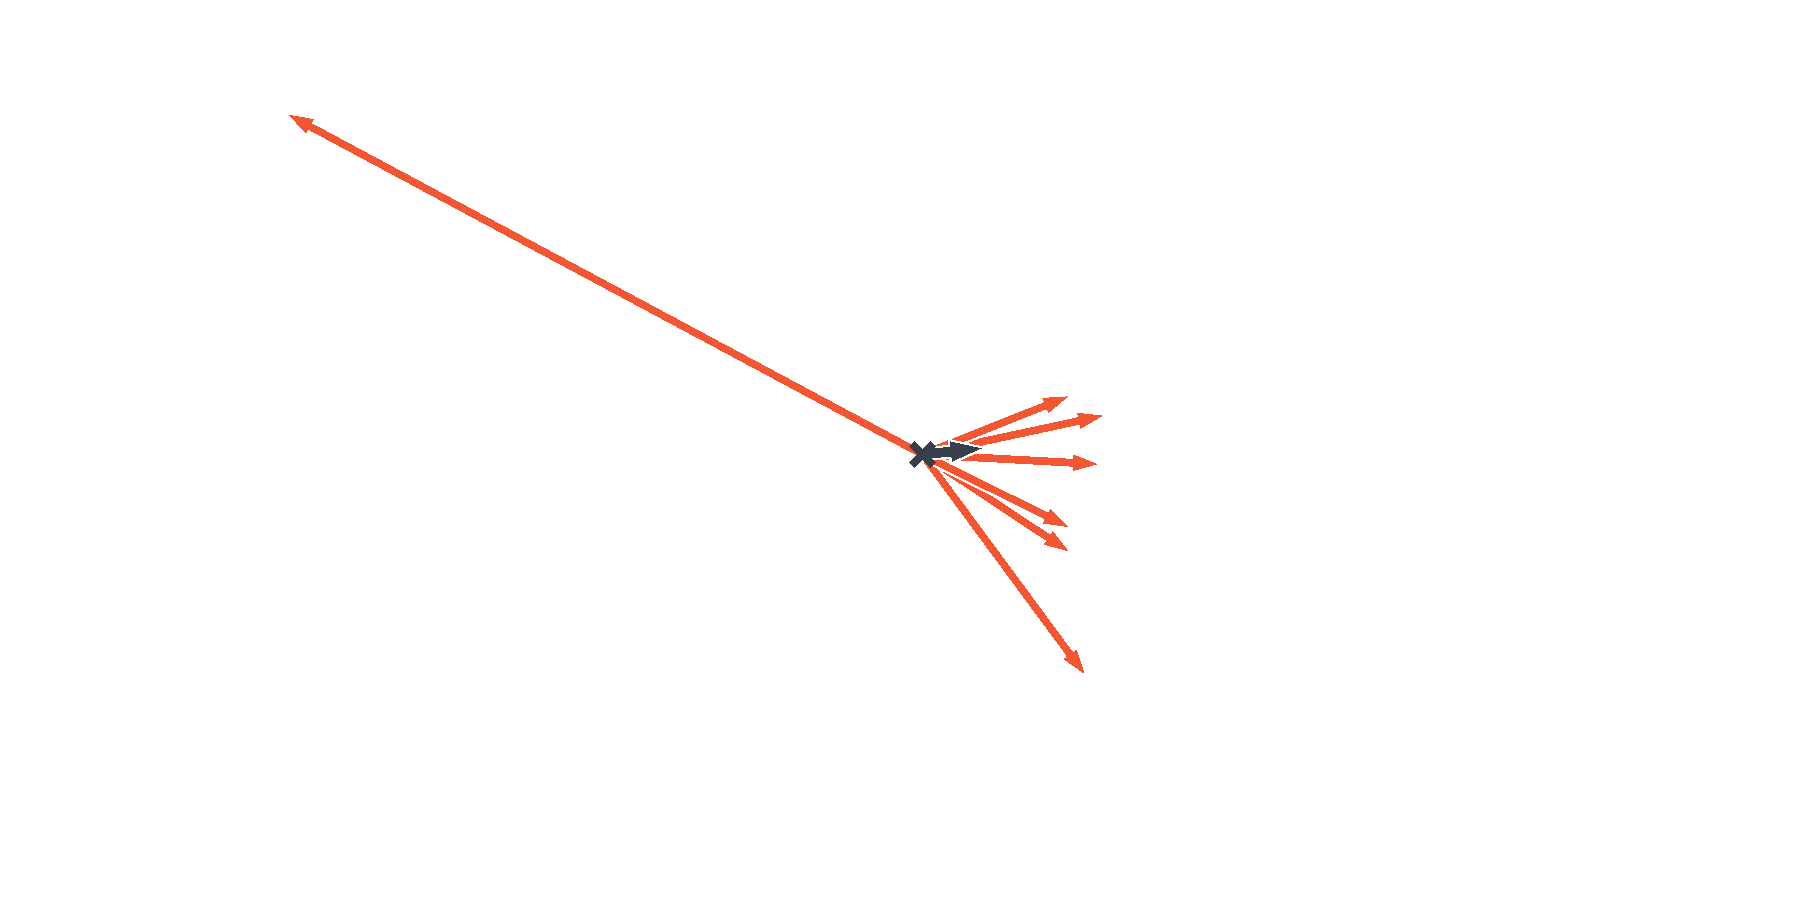
\includegraphics[width=\linewidth, trim={4.8cm 3.8cm 11.3cm 1.9cm}, clip]{../repos/backpack-paper/code/animations/differential-privacy/dp_frame_0}
    \caption{Individual gradients}\label{subfig:background::DifferentialPrivacy1}
  \end{subfigure}
  \begin{subfigure}{0.495\linewidth}
    % trim={<left> <lower> <right> <upper>}, clip
    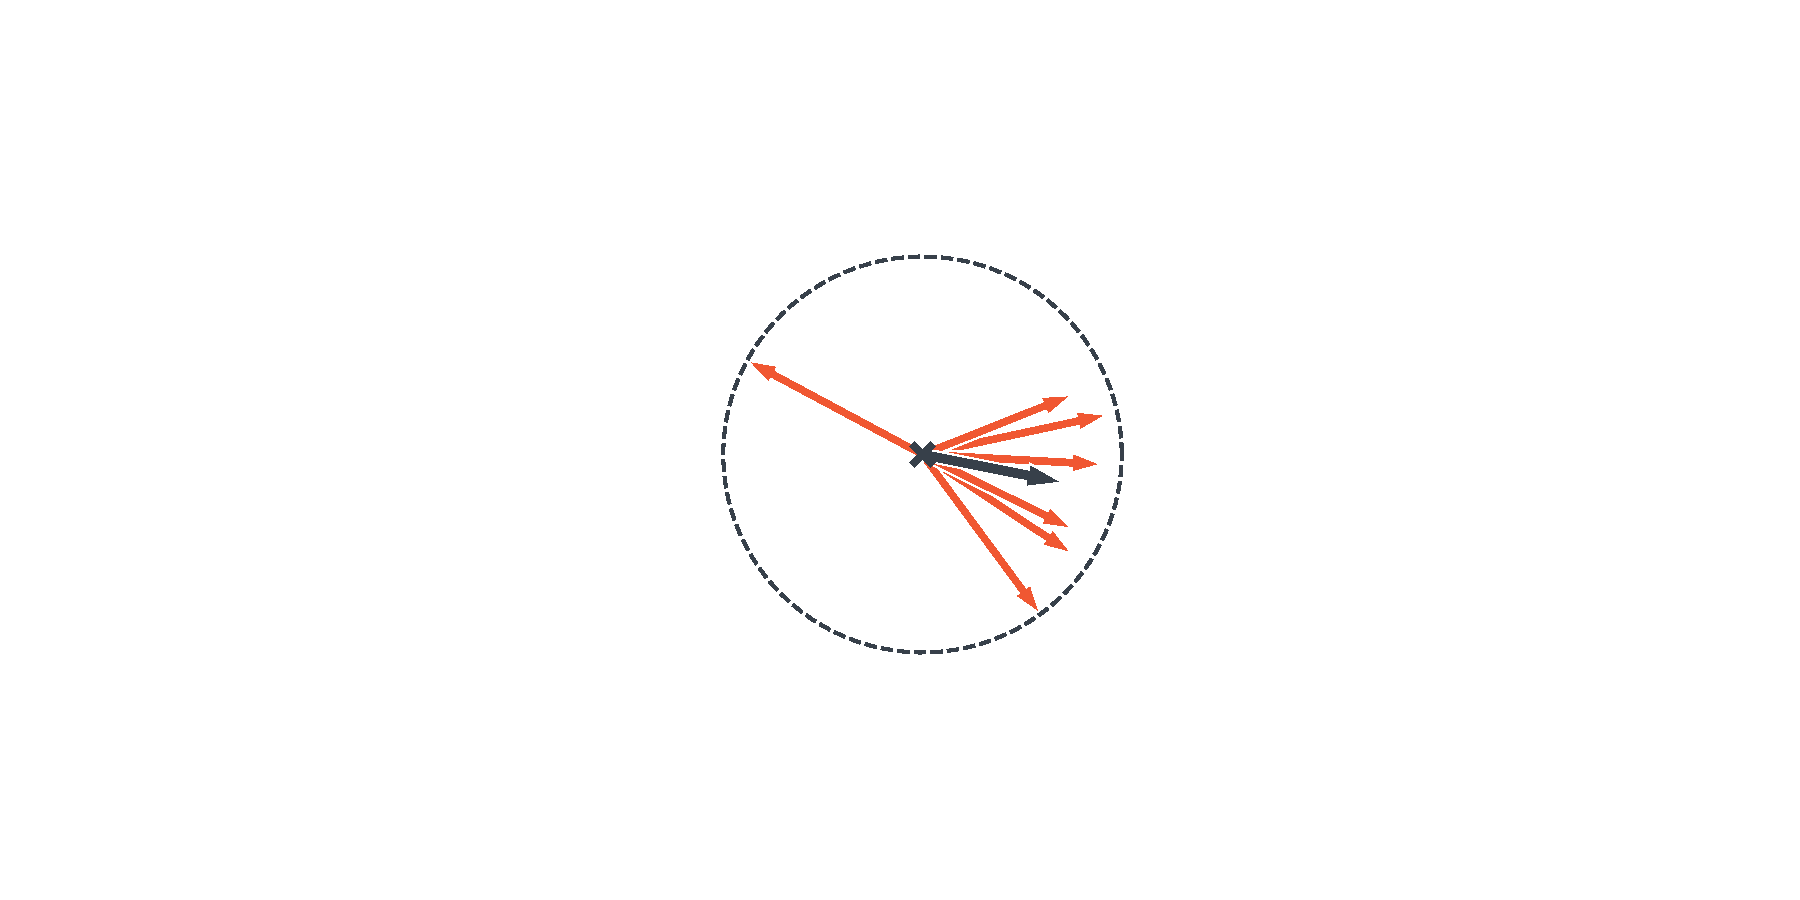
\includegraphics[width=\linewidth, trim={4.8cm 3.8cm 11.3cm 1.9cm}, clip]{../repos/backpack-paper/code/animations/differential-privacy/dp_frame_4}
    \caption{Clipped individual
      gradients}\label{subfig:background::DifferentialPrivacy2}
  \end{subfigure}
  \caption{\textbf{(Sketch) DP-SGD requires access to per-sample gradients.}
    \subfigref{subfig:background::DifferentialPrivacy1} The average gradient
    (black arrow) might be dominated by the per-sample gradients (orange arrows)
    of a small number of data. Adversaries might use this to extract potentially
    sensitive information about that data.
    \subfigref{subfig:background::DifferentialPrivacy2} Clipping per-sample
    gradients before averaging them limits the influence of individual data. The
    dashed circle's radius corresponds to the privacy threshold $C$.
  }\label{fig:background::DifferentialPrivacy}
\end{figure}

One prominent example for deep learning is differentially-private SGD
(DP-SGD)~\cite[Algorithm 1]{abadi2016deep}, which uses a negative average of
processed individual gradients over a mini-batch. To bound the influence of
individual data, per-sample gradients whose norm exceeds a specific threshold
$C$ are clipped back to norm $C$ (\Cref{fig:background::DifferentialPrivacy}),
\begin{align*}
  \vgtilde_n(\vtheta_t)
  =
  \frac{
  \vg_n(\vtheta_t)
  }{
  \max\left(
  1,
  \frac{\lVert \vg_n(\vtheta_t) \rVert_2}{C}
  \right)
  }\,.
\end{align*}
Gaussian noise of scale $\sigma$ is then added to each gradient,
\begin{align*}
  \vghat_n(\vtheta_t)
  =
  \vgtilde_n(\vtheta_t) + \vepsilon_n\,,
  \qquad
  \vepsilon_n \sim \gN(\vzero, {(\sigma C)}^2 \mI)\,.
\end{align*}
DP-SGD performs the update rule of SGD, with $\vg_n$ replaced by
$\vghat_n$,
\begin{align*}
  \vtheta_{t+1}
  =
  \vtheta_t
  -
  \eta_t
  \frac{1}{|\sB|}
  \sum_{(\vx_n,\vy_n) \in \sB}
  \vghat_n(\vtheta_t)\,.
\end{align*}
This requires access to per-sample gradient norms $\{\lVert \vg_n(\vtheta_t)
\rVert_2\}_{n}$.

\subsection{Importance Sampling}

\marginnote[*-22]{
  \begin{center}
    \pgfkeys{/pgfplots/BackPACKImportanceSamplingMNIST/.style={
    xmin = -0.02,
    xmax = 1.02,
    xtick={0, 1},
    xticklabels = {0, max},
    xlabel={$\lVert \nabla_{\vtheta}\ell_{n} \rVert_2$},
    scaled y ticks=real:50000,
    y tick label style={
      /pgf/number format/.cd,
      fixed,
      fixed zerofill,
      precision=2,
      /tikz/.cd
    },
    ytick scale label code/.code={$\cdot |\sD_{\text{train}}|$},
    ylabel = {},
    width = 1.15\linewidth,
    height = 0.9\linewidth,
    every axis plot/.append style={line width = 1.5pt},
    axis line style = black,
    tick pos = left,
    xtick align = inside,
    ytick align = inside,
    xmajorticks = true,
    ymajorticks = true,
    ylabel near ticks,
    xlabel near ticks,
    xticklabel style = {font = \footnotesize},
    xlabel style = {font = \footnotesize},
    yticklabel style = {font = \footnotesize},
    ylabel style = {font = \footnotesize},
    title style = {font = \footnotesize},
    grid = major,
    grid style = {dashed},
    legend cell align = left,
    legend style = {
      fill opacity = 0,
      text opacity = 0,
      draw opacity = 0,
      font = \footnotesize,
    },
  }
}

%%% Local Variables:
%%% mode: latex
%%% TeX-master: "../../thesis"
%%% End:

    \captionsetup[sub]{labelformat=parens}
    \begingroup
    \captionsetup{type=figure}
    \begin{subfigure}{\linewidth}
      \caption{Epoch 0, train accuracy 9.83\%}
      \vspace{-1ex}
      \pgfkeys{/pgfplots/zmystyle/.style={
          BackPACKImportanceSamplingMNIST,
          xlabel = \empty,
          xticklabel style = {opacity = 0},
        }
      }
      \tikzexternalenable
      % This file was created by tikzplotlib v0.9.0.
\begin{tikzpicture}

\definecolor{color0}{rgb}{0.941176470588235,0.341176470588235,0.196078431372549}

\begin{axis}[
axis line style={white!80!black},
legend cell align={left},
legend style={fill opacity=0.8, draw opacity=1, text opacity=1, draw=white!80!black},
tick pos=left,
x grid style={white!80!black},
xmin=0.180960892984677, xmax=1.03900186223882,
xtick style={color=gray},
xtick={0.1,0.2,0.3,0.4,0.5,0.6,0.7,0.8,0.9,1,1.1},
xticklabels={0.1,0.2,0.3,0.4,0.5,0.6,0.7,0.8,0.9,1.0,1.1},
y grid style={white!80!black},
ymin=0, ymax=3290.7,
ytick style={color=gray},
zmystyle
]
\draw[draw=white,fill=color0] (axis cs:0.219962755223502,0) rectangle (axis cs:0.235563500119032,4);
\addlegendimage{ybar,ybar legend,draw=white,fill=color0};
\addlegendentry{\ Epoch: 00, accuracy: 09.83\%}

\draw[draw=white,fill=color0] (axis cs:0.235563500119032,0) rectangle (axis cs:0.251164245014562,7);
\draw[draw=white,fill=color0] (axis cs:0.251164245014562,0) rectangle (axis cs:0.266764989910092,25);
\draw[draw=white,fill=color0] (axis cs:0.266764989910092,0) rectangle (axis cs:0.282365734805622,43);
\draw[draw=white,fill=color0] (axis cs:0.282365734805622,0) rectangle (axis cs:0.297966479701152,79);
\draw[draw=white,fill=color0] (axis cs:0.297966479701152,0) rectangle (axis cs:0.313567224596682,139);
\draw[draw=white,fill=color0] (axis cs:0.313567224596682,0) rectangle (axis cs:0.329167969492212,265);
\draw[draw=white,fill=color0] (axis cs:0.329167969492212,0) rectangle (axis cs:0.344768714387742,394);
\draw[draw=white,fill=color0] (axis cs:0.344768714387742,0) rectangle (axis cs:0.360369459283272,573);
\draw[draw=white,fill=color0] (axis cs:0.360369459283272,0) rectangle (axis cs:0.375970204178802,792);
\draw[draw=white,fill=color0] (axis cs:0.375970204178802,0) rectangle (axis cs:0.391570949074331,1008);
\draw[draw=white,fill=color0] (axis cs:0.391570949074332,0) rectangle (axis cs:0.407171693969862,1279);
\draw[draw=white,fill=color0] (axis cs:0.407171693969862,0) rectangle (axis cs:0.422772438865392,1519);
\draw[draw=white,fill=color0] (axis cs:0.422772438865392,0) rectangle (axis cs:0.438373183760921,1738);
\draw[draw=white,fill=color0] (axis cs:0.438373183760921,0) rectangle (axis cs:0.453973928656451,2090);
\draw[draw=white,fill=color0] (axis cs:0.453973928656451,0) rectangle (axis cs:0.469574673551981,2418);
\draw[draw=white,fill=color0] (axis cs:0.469574673551981,0) rectangle (axis cs:0.485175418447511,2540);
\draw[draw=white,fill=color0] (axis cs:0.485175418447511,0) rectangle (axis cs:0.500776163343041,2808);
\draw[draw=white,fill=color0] (axis cs:0.500776163343041,0) rectangle (axis cs:0.516376908238571,2924);
\draw[draw=white,fill=color0] (axis cs:0.516376908238571,0) rectangle (axis cs:0.531977653134101,3085);
\draw[draw=white,fill=color0] (axis cs:0.531977653134101,0) rectangle (axis cs:0.547578398029631,3063);
\draw[draw=white,fill=color0] (axis cs:0.547578398029631,0) rectangle (axis cs:0.563179142925161,3134);
\draw[draw=white,fill=color0] (axis cs:0.563179142925161,0) rectangle (axis cs:0.578779887820691,2925);
\draw[draw=white,fill=color0] (axis cs:0.578779887820691,0) rectangle (axis cs:0.594380632716221,2761);
\draw[draw=white,fill=color0] (axis cs:0.594380632716221,0) rectangle (axis cs:0.609981377611751,2560);
\draw[draw=white,fill=color0] (axis cs:0.609981377611751,0) rectangle (axis cs:0.625582122507281,2211);
\draw[draw=white,fill=color0] (axis cs:0.625582122507281,0) rectangle (axis cs:0.641182867402811,1927);
\draw[draw=white,fill=color0] (axis cs:0.641182867402811,0) rectangle (axis cs:0.656783612298341,1669);
\draw[draw=white,fill=color0] (axis cs:0.656783612298341,0) rectangle (axis cs:0.672384357193871,1476);
\draw[draw=white,fill=color0] (axis cs:0.672384357193871,0) rectangle (axis cs:0.687985102089401,1118);
\draw[draw=white,fill=color0] (axis cs:0.687985102089401,0) rectangle (axis cs:0.703585846984931,925);
\draw[draw=white,fill=color0] (axis cs:0.703585846984931,0) rectangle (axis cs:0.719186591880461,673);
\draw[draw=white,fill=color0] (axis cs:0.719186591880461,0) rectangle (axis cs:0.734787336775991,511);
\draw[draw=white,fill=color0] (axis cs:0.734787336775991,0) rectangle (axis cs:0.750388081671521,411);
\draw[draw=white,fill=color0] (axis cs:0.750388081671521,0) rectangle (axis cs:0.765988826567051,257);
\draw[draw=white,fill=color0] (axis cs:0.765988826567051,0) rectangle (axis cs:0.781589571462581,174);
\draw[draw=white,fill=color0] (axis cs:0.781589571462581,0) rectangle (axis cs:0.797190316358111,154);
\draw[draw=white,fill=color0] (axis cs:0.797190316358111,0) rectangle (axis cs:0.812791061253641,91);
\draw[draw=white,fill=color0] (axis cs:0.812791061253641,0) rectangle (axis cs:0.828391806149171,54);
\draw[draw=white,fill=color0] (axis cs:0.82839180614917,0) rectangle (axis cs:0.8439925510447,40);
\draw[draw=white,fill=color0] (axis cs:0.8439925510447,0) rectangle (axis cs:0.85959329594023,17);
\draw[draw=white,fill=color0] (axis cs:0.85959329594023,0) rectangle (axis cs:0.87519404083576,20);
\draw[draw=white,fill=color0] (axis cs:0.87519404083576,0) rectangle (axis cs:0.89079478573129,9);
\draw[draw=white,fill=color0] (axis cs:0.89079478573129,0) rectangle (axis cs:0.90639553062682,4);
\draw[draw=white,fill=color0] (axis cs:0.90639553062682,0) rectangle (axis cs:0.92199627552235,2);
\draw[draw=white,fill=color0] (axis cs:0.92199627552235,0) rectangle (axis cs:0.93759702041788,1);
\draw[draw=white,fill=color0] (axis cs:0.93759702041788,0) rectangle (axis cs:0.95319776531341,2);
\draw[draw=white,fill=color0] (axis cs:0.95319776531341,0) rectangle (axis cs:0.96879851020894,0);
\draw[draw=white,fill=color0] (axis cs:0.96879851020894,0) rectangle (axis cs:0.98439925510447,0);
\draw[draw=white,fill=color0] (axis cs:0.98439925510447,0) rectangle (axis cs:1,1);
\end{axis}

\end{tikzpicture}

      \tikzexternaldisable
      \vspace{-6ex}
    \end{subfigure}
    \begin{subfigure}{\linewidth}
      \caption{Epoch 2, train accuracy 83.4\%}
      \vspace{-1ex}
      \pgfkeys{/pgfplots/zmystyle/.style={
          BackPACKImportanceSamplingMNIST,
          xlabel = \empty,
          xticklabel style = {opacity = 0},
        }
      }
      \tikzexternalenable
      % This file was created by tikzplotlib v0.9.0.
\begin{tikzpicture}

\definecolor{color0}{rgb}{0.941176470588235,0.341176470588235,0.196078431372549}

\begin{axis}[
axis line style={white!80!black},
legend cell align={left},
legend style={fill opacity=0.8, draw opacity=1, text opacity=1, draw=white!80!black},
tick pos=left,
x grid style={white!80!black},
xmin=-0.0235874482194031, xmax=1.04874225943902,
xtick style={color=gray},
xtick={-0.2,0,0.2,0.4,0.6,0.8,1,1.2},
xticklabels={−0.2,0.0,0.2,0.4,0.6,0.8,1.0,1.2},
y grid style={white!80!black},
ymin=0, ymax=3099.6,
ytick style={color=gray},
zmystyle
]
\draw[draw=white,fill=color0] (axis cs:0.0251548112196161,0) rectangle (axis cs:0.0446517149952238,90);
\addlegendimage{ybar,ybar legend,draw=white,fill=color0};
\addlegendentry{\ Epoch: 02, accuracy: 83.40\%}

\draw[draw=white,fill=color0] (axis cs:0.0446517149952238,0) rectangle (axis cs:0.0641486187708315,293);
\draw[draw=white,fill=color0] (axis cs:0.0641486187708315,0) rectangle (axis cs:0.0836455225464392,611);
\draw[draw=white,fill=color0] (axis cs:0.0836455225464392,0) rectangle (axis cs:0.103142426322047,1523);
\draw[draw=white,fill=color0] (axis cs:0.103142426322047,0) rectangle (axis cs:0.122639330097655,1968);
\draw[draw=white,fill=color0] (axis cs:0.122639330097655,0) rectangle (axis cs:0.142136233873262,1998);
\draw[draw=white,fill=color0] (axis cs:0.142136233873262,0) rectangle (axis cs:0.16163313764887,1973);
\draw[draw=white,fill=color0] (axis cs:0.16163313764887,0) rectangle (axis cs:0.181130041424478,2001);
\draw[draw=white,fill=color0] (axis cs:0.181130041424478,0) rectangle (axis cs:0.200626945200085,2081);
\draw[draw=white,fill=color0] (axis cs:0.200626945200085,0) rectangle (axis cs:0.220123848975693,2047);
\draw[draw=white,fill=color0] (axis cs:0.220123848975693,0) rectangle (axis cs:0.239620752751301,2217);
\draw[draw=white,fill=color0] (axis cs:0.239620752751301,0) rectangle (axis cs:0.259117656526908,2397);
\draw[draw=white,fill=color0] (axis cs:0.259117656526908,0) rectangle (axis cs:0.278614560302516,2682);
\draw[draw=white,fill=color0] (axis cs:0.278614560302516,0) rectangle (axis cs:0.298111464078124,2769);
\draw[draw=white,fill=color0] (axis cs:0.298111464078124,0) rectangle (axis cs:0.317608367853731,2952);
\draw[draw=white,fill=color0] (axis cs:0.317608367853731,0) rectangle (axis cs:0.337105271629339,2754);
\draw[draw=white,fill=color0] (axis cs:0.337105271629339,0) rectangle (axis cs:0.356602175404947,2654);
\draw[draw=white,fill=color0] (axis cs:0.356602175404947,0) rectangle (axis cs:0.376099079180554,2566);
\draw[draw=white,fill=color0] (axis cs:0.376099079180554,0) rectangle (axis cs:0.395595982956162,2335);
\draw[draw=white,fill=color0] (axis cs:0.395595982956162,0) rectangle (axis cs:0.41509288673177,2063);
\draw[draw=white,fill=color0] (axis cs:0.41509288673177,0) rectangle (axis cs:0.434589790507377,1800);
\draw[draw=white,fill=color0] (axis cs:0.434589790507377,0) rectangle (axis cs:0.454086694282985,1570);
\draw[draw=white,fill=color0] (axis cs:0.454086694282985,0) rectangle (axis cs:0.473583598058593,1361);
\draw[draw=white,fill=color0] (axis cs:0.473583598058593,0) rectangle (axis cs:0.4930805018342,1056);
\draw[draw=white,fill=color0] (axis cs:0.4930805018342,0) rectangle (axis cs:0.512577405609808,891);
\draw[draw=white,fill=color0] (axis cs:0.512577405609808,0) rectangle (axis cs:0.532074309385416,730);
\draw[draw=white,fill=color0] (axis cs:0.532074309385416,0) rectangle (axis cs:0.551571213161023,567);
\draw[draw=white,fill=color0] (axis cs:0.551571213161023,0) rectangle (axis cs:0.571068116936631,437);
\draw[draw=white,fill=color0] (axis cs:0.571068116936631,0) rectangle (axis cs:0.590565020712239,347);
\draw[draw=white,fill=color0] (axis cs:0.590565020712239,0) rectangle (axis cs:0.610061924487846,290);
\draw[draw=white,fill=color0] (axis cs:0.610061924487846,0) rectangle (axis cs:0.629558828263454,207);
\draw[draw=white,fill=color0] (axis cs:0.629558828263454,0) rectangle (axis cs:0.649055732039062,195);
\draw[draw=white,fill=color0] (axis cs:0.649055732039062,0) rectangle (axis cs:0.66855263581467,138);
\draw[draw=white,fill=color0] (axis cs:0.668552635814669,0) rectangle (axis cs:0.688049539590277,106);
\draw[draw=white,fill=color0] (axis cs:0.688049539590277,0) rectangle (axis cs:0.707546443365885,67);
\draw[draw=white,fill=color0] (axis cs:0.707546443365885,0) rectangle (axis cs:0.727043347141493,54);
\draw[draw=white,fill=color0] (axis cs:0.727043347141493,0) rectangle (axis cs:0.7465402509171,35);
\draw[draw=white,fill=color0] (axis cs:0.7465402509171,0) rectangle (axis cs:0.766037154692708,35);
\draw[draw=white,fill=color0] (axis cs:0.766037154692708,0) rectangle (axis cs:0.785534058468316,13);
\draw[draw=white,fill=color0] (axis cs:0.785534058468316,0) rectangle (axis cs:0.805030962243923,16);
\draw[draw=white,fill=color0] (axis cs:0.805030962243923,0) rectangle (axis cs:0.824527866019531,14);
\draw[draw=white,fill=color0] (axis cs:0.824527866019531,0) rectangle (axis cs:0.844024769795139,4);
\draw[draw=white,fill=color0] (axis cs:0.844024769795139,0) rectangle (axis cs:0.863521673570746,5);
\draw[draw=white,fill=color0] (axis cs:0.863521673570746,0) rectangle (axis cs:0.883018577346354,2);
\draw[draw=white,fill=color0] (axis cs:0.883018577346354,0) rectangle (axis cs:0.902515481121962,2);
\draw[draw=white,fill=color0] (axis cs:0.902515481121962,0) rectangle (axis cs:0.922012384897569,1);
\draw[draw=white,fill=color0] (axis cs:0.922012384897569,0) rectangle (axis cs:0.941509288673177,0);
\draw[draw=white,fill=color0] (axis cs:0.941509288673177,0) rectangle (axis cs:0.961006192448785,0);
\draw[draw=white,fill=color0] (axis cs:0.961006192448785,0) rectangle (axis cs:0.980503096224392,2);
\draw[draw=white,fill=color0] (axis cs:0.980503096224392,0) rectangle (axis cs:1,1);
\end{axis}

\end{tikzpicture}

      \tikzexternaldisable
      \vspace{-6ex}
    \end{subfigure}
    \begin{subfigure}{\linewidth}
      \caption{Epoch 49, train accuracy 90.5\%}
      \vspace{-1ex}
      \pgfkeys{/pgfplots/zmystyle/.style={
          BackPACKImportanceSamplingMNIST,
        }
      }
      \tikzexternalenable
      % This file was created by tikzplotlib v0.9.0.
\begin{tikzpicture}

\definecolor{color0}{rgb}{0.941176470588235,0.341176470588235,0.196078431372549}

\begin{axis}[
axis line style={white!80!black},
legend cell align={left},
legend style={fill opacity=0.8, draw opacity=1, text opacity=1, draw=white!80!black},
tick pos=left,
x grid style={white!80!black},
xmin=-0.0499953146370904, xmax=1.04999977688748,
xtick style={color=gray},
xtick={-0.2,0,0.2,0.4,0.6,0.8,1,1.2},
xticklabels={−0.2,0.0,0.2,0.4,0.6,0.8,1.0,1.2},
y grid style={white!80!black},
ymin=0, ymax=20526.45,
ytick style={color=gray},
zmystyle
]
\draw[draw=white,fill=color0] (axis cs:4.46225039008562e-06,0) rectangle (axis cs:0.0200043730053823,19549);
\addlegendimage{ybar,ybar legend,draw=white,fill=color0};
\addlegendentry{\ Epoch: 49, accuracy: 90.49\%}

\draw[draw=white,fill=color0] (axis cs:0.0200043730053823,0) rectangle (axis cs:0.0400042837603745,7018);
\draw[draw=white,fill=color0] (axis cs:0.0400042837603745,0) rectangle (axis cs:0.0600041945153667,4100);
\draw[draw=white,fill=color0] (axis cs:0.0600041945153667,0) rectangle (axis cs:0.0800041052703589,2853);
\draw[draw=white,fill=color0] (axis cs:0.0800041052703589,0) rectangle (axis cs:0.100004016025351,2112);
\draw[draw=white,fill=color0] (axis cs:0.100004016025351,0) rectangle (axis cs:0.120003926780343,1752);
\draw[draw=white,fill=color0] (axis cs:0.120003926780343,0) rectangle (axis cs:0.140003837535335,1514);
\draw[draw=white,fill=color0] (axis cs:0.140003837535335,0) rectangle (axis cs:0.160003748290328,1212);
\draw[draw=white,fill=color0] (axis cs:0.160003748290328,0) rectangle (axis cs:0.18000365904532,1032);
\draw[draw=white,fill=color0] (axis cs:0.18000365904532,0) rectangle (axis cs:0.200003569800312,866);
\draw[draw=white,fill=color0] (axis cs:0.200003569800312,0) rectangle (axis cs:0.220003480555304,810);
\draw[draw=white,fill=color0] (axis cs:0.220003480555304,0) rectangle (axis cs:0.240003391310296,694);
\draw[draw=white,fill=color0] (axis cs:0.240003391310296,0) rectangle (axis cs:0.260003302065289,661);
\draw[draw=white,fill=color0] (axis cs:0.260003302065289,0) rectangle (axis cs:0.280003212820281,594);
\draw[draw=white,fill=color0] (axis cs:0.280003212820281,0) rectangle (axis cs:0.300003123575273,537);
\draw[draw=white,fill=color0] (axis cs:0.300003123575273,0) rectangle (axis cs:0.320003034330265,521);
\draw[draw=white,fill=color0] (axis cs:0.320003034330265,0) rectangle (axis cs:0.340002945085257,462);
\draw[draw=white,fill=color0] (axis cs:0.340002945085257,0) rectangle (axis cs:0.36000285584025,415);
\draw[draw=white,fill=color0] (axis cs:0.36000285584025,0) rectangle (axis cs:0.380002766595242,391);
\draw[draw=white,fill=color0] (axis cs:0.380002766595242,0) rectangle (axis cs:0.400002677350234,384);
\draw[draw=white,fill=color0] (axis cs:0.400002677350234,0) rectangle (axis cs:0.420002588105226,341);
\draw[draw=white,fill=color0] (axis cs:0.420002588105226,0) rectangle (axis cs:0.440002498860218,325);
\draw[draw=white,fill=color0] (axis cs:0.440002498860218,0) rectangle (axis cs:0.460002409615211,271);
\draw[draw=white,fill=color0] (axis cs:0.460002409615211,0) rectangle (axis cs:0.480002320370203,261);
\draw[draw=white,fill=color0] (axis cs:0.480002320370203,0) rectangle (axis cs:0.500002231125195,230);
\draw[draw=white,fill=color0] (axis cs:0.500002231125195,0) rectangle (axis cs:0.520002141880187,188);
\draw[draw=white,fill=color0] (axis cs:0.520002141880187,0) rectangle (axis cs:0.54000205263518,160);
\draw[draw=white,fill=color0] (axis cs:0.54000205263518,0) rectangle (axis cs:0.560001963390172,123);
\draw[draw=white,fill=color0] (axis cs:0.560001963390172,0) rectangle (axis cs:0.580001874145164,129);
\draw[draw=white,fill=color0] (axis cs:0.580001874145164,0) rectangle (axis cs:0.600001784900156,92);
\draw[draw=white,fill=color0] (axis cs:0.600001784900156,0) rectangle (axis cs:0.620001695655148,73);
\draw[draw=white,fill=color0] (axis cs:0.620001695655148,0) rectangle (axis cs:0.64000160641014,67);
\draw[draw=white,fill=color0] (axis cs:0.64000160641014,0) rectangle (axis cs:0.660001517165133,50);
\draw[draw=white,fill=color0] (axis cs:0.660001517165133,0) rectangle (axis cs:0.680001427920125,32);
\draw[draw=white,fill=color0] (axis cs:0.680001427920125,0) rectangle (axis cs:0.700001338675117,26);
\draw[draw=white,fill=color0] (axis cs:0.700001338675117,0) rectangle (axis cs:0.720001249430109,31);
\draw[draw=white,fill=color0] (axis cs:0.720001249430109,0) rectangle (axis cs:0.740001160185101,15);
\draw[draw=white,fill=color0] (axis cs:0.740001160185102,0) rectangle (axis cs:0.760001070940094,9);
\draw[draw=white,fill=color0] (axis cs:0.760001070940094,0) rectangle (axis cs:0.780000981695086,7);
\draw[draw=white,fill=color0] (axis cs:0.780000981695086,0) rectangle (axis cs:0.800000892450078,6);
\draw[draw=white,fill=color0] (axis cs:0.800000892450078,0) rectangle (axis cs:0.82000080320507,1);
\draw[draw=white,fill=color0] (axis cs:0.82000080320507,0) rectangle (axis cs:0.840000713960062,1);
\draw[draw=white,fill=color0] (axis cs:0.840000713960062,0) rectangle (axis cs:0.860000624715055,0);
\draw[draw=white,fill=color0] (axis cs:0.860000624715055,0) rectangle (axis cs:0.880000535470047,2);
\draw[draw=white,fill=color0] (axis cs:0.880000535470047,0) rectangle (axis cs:0.900000446225039,0);
\draw[draw=white,fill=color0] (axis cs:0.900000446225039,0) rectangle (axis cs:0.920000356980031,0);
\draw[draw=white,fill=color0] (axis cs:0.920000356980031,0) rectangle (axis cs:0.940000267735023,2);
\draw[draw=white,fill=color0] (axis cs:0.940000267735023,0) rectangle (axis cs:0.960000178490016,0);
\draw[draw=white,fill=color0] (axis cs:0.960000178490016,0) rectangle (axis cs:0.980000089245008,0);
\draw[draw=white,fill=color0] (axis cs:0.980000089245008,0) rectangle (axis cs:1,1);
\end{axis}

\end{tikzpicture}

      \tikzexternaldisable
      \vspace{-2ex}
    \end{subfigure}
    \endgroup
    \captionof{figure}{\textbf{Importance distribution of samples during
        training.} Importance is measured by individual gradient $L_{2}$ norms,
      computed with \backpack (\Cref{chap:backpack}). As training proceeds and
      more examples are correctly classified and become ``unimportant''.
      Details: logistic regression on \mnist, trained with \sgd, $|\sB| = 128$,
      and learning rate $0.005$.}\label{fig:background::SquaredL2Norms}
  \end{center}
}

A hypothesis about learning in ML is that the model first learns to correctly
predict ``easy'' examples. Only in later phases are the ``difficult'' examples
learned. Using these harder examples more frequently for training might help
speed up the learning procedure. Put differently, some data matter more at
certain stages of training than other, which is quantified through a measure of
importance. Importance sampling realizes this idea of selecting important data
more frequently. It does so by adapting the sampling procedure for mini-batches
to reduce the gradient variance, which beneficially influences the convergence
of stochastic first-order methods like \sgd, and therefore speeds up training. A
common strategy is to weight the importance of samples by the per-sample $L_2$
norm
(\Cref{eq:background::importanceSamplingOptimalDistribution,fig:background::SquaredL2Norms}).

As a starting point to see how the sampling procedure affects optimization,
consider the generalization of uniform sampling from
\Cref{sec:background::MiniBatching} for $|\sB| = 1$. At training iteration $t$,
a sample $n_t\sim p_t(n_t)$ is drawn from a current sampling distribution
$p_t(n_t)$ over $\{1, \dots, |\sD|\}$. \sgd with a learning rate $\eta$ uses the
unbiased gradient estimator\sidenote[][0\baselineskip]{%
  For uniform sampling $p_{t}(n_{t}) = \nicefrac{1}{|\sD|}$, which is the most
  common case in practice, the scaling factor cancels and yields the commonly
  used gradient estimator that would be used by ``normal'' \sgd with $|\sB| =
  1$.%
}
\begin{subequations}
  \begin{align}\label{eq:background::gradientEstimator}
    \vghat_{n_t}(\vtheta_t)
    &:=
      \frac{1}{|\sD| p_t(n_t)}
      \grad{\vtheta_t}\ell_{n_t}(\vtheta_t)
      \shortintertext{with}
      \E_{n_t \sim p_t(n_t)}\left[ \vghat_{n_t}(\vtheta_t) \right]
    &=
      \frac{1}{|\sD|} \sum_{(\vx_n, \vy_n) \in \sD}
      \grad{\vtheta_t} \ell_{n_t}(\vtheta_t)
      = \vg_{\sD}(\vtheta_t)
      \shortintertext{to update the parameters}
      \label{eq:background::gradientDescentSampled}
      \vtheta_{t+1} &= \vtheta_t - \eta \vghat_{n_t}(\vtheta_{t})\,.
  \end{align}
\end{subequations}
Using a non-uniform distribution over stochastic gradients would introduce bias
in the update, so in importance sampling the samples are weighted by their
probability of being selected to undo the bias. The distribution can then be
tuned to minimize the variance of the estimator and improve performance: one can
assess convergence of \Cref{eq:background::gradientDescentSampled} through the
progress towards the minimizer $\vtheta_{\star}$ in terms of squared $L_2$
distance~\cite{wang2017accelerating,katharopoulos2018samples},
\begin{subequations}
  \begin{align}
    \lVert \vtheta_{t} - \vtheta_{\star} \rVert_2^{2}
    -
    \lVert \vtheta_{t+1} - \vtheta_{\star} \rVert_2^{2}\,.
  \end{align}
  In expectation, this measure of convergence depends on the gradient estimator's
  variance (more specifically, its trace),
  \begin{align}
    \begin{split}
      \E_{n_t}
      &\left[
        \lVert \vtheta_{t} - \vtheta_{\star} \rVert_2^2
        -
        \lVert \vtheta_{t+1} - \vtheta_{\star} \rVert_2^2
        \right]
      \\
      &=
        \E_{n_t}\left[
        \lVert \vtheta_{t} - \vtheta_{\star} \rVert_2^{2}
        -
        \lVert \vtheta_{t} - \vtheta_{\star} - \eta \vghat_{n_t}  \rVert_2^{2}
        \right]
      \\
      &=
        \E_{n_t}\left[
        2 \eta \left(
        \vtheta_{t} - \vtheta_{\star}
        \right)^{\top} \vghat_{n_t}
        - \eta^2 \vghat_{n_t}^{\top} \vghat_{n_t}
        \right]
      \\
      &=
        2 \eta \left(
        \vtheta_{t} - \vtheta_{\star}
        \right)^{\top}
        \vg_{\sD}
        -
        \eta^2 \E_{n_t}\left[
        \lVert \vghat_{n_t} \rVert_2^2
        \right]
      \\
      &=
        2 \eta \left(
        \vtheta_{t} - \vtheta_{\star}
        \right)^{\top}
        \vg_{\sD}
        - \eta^2 \lVert \vg_{\sD} \rVert_2^2
        -
        \eta^2 \E_{n_t}\left[
        \lVert \vghat_{n_t} - \vg_{\sD} \rVert_2^2
        \right]
      \\
      &=
        2 \eta \left(
        \vtheta_{t} - \vtheta_{\star}
        \right)^{\top}
        \vg_{\sD}
        - \eta^2 \lVert \vg_{\sD} \rVert_2^2
        -
        \eta^2 \Tr\left\{
        \Var_{n_t}\left[\vghat_{n_t}
        \right]\right\}
    \end{split}
  \end{align}
\end{subequations}
For what follows, the intuition is that sampling affects convergence through the
variance term, and minimizing this term improves convergence. Hence, the goal is
to identify the optimal sampling via
\begin{align}\label{ex:background::findOptimalSamplingDistribution}
  \minimize_{\substack{p_t(n_t) \\ \sum_{n=1}^{|\sD|} p_t(n) = 1}}
  \Tr\left\{
  \Var_{n_t}\left[\vghat_{n_t}
  \right]\right\}
  \quad
  \Leftrightarrow
  \quad
  \minimize_{\substack{p_t(n_t) \\ \sum_{n=1}^{|\sD|} p_t(n) = 1}}
  \E_{n_t}
  \left[
  \lVert
  \vghat_{n_t}
  \rVert_2^2
  \right]
\end{align}
The solution, outlined in \Cref{ex:background::importanceSamplingDerivation}, is
\begin{align}
  \label{eq:background::importanceSamplingOptimalDistribution}
  p_t(n_t)
  =
  \frac{
  \lVert \grad{\vtheta_t}\ell_{n_t}(\vtheta_t) \rVert_2
  }{
  \sum_{n=1}^{|\sD|} \lVert \ell_{n}(\vtheta_t) \rVert_2
  }\,.
\end{align}
%
and
\marginnote[*-31]{%
  \begin{remark}[\textbf{Optimal sampling
      distribution~\cite{needell2014stochastic,zhao2015stochastic}}]\label{ex:background::importanceSamplingDerivation}
    (The iteration index $t$ is suppressed for brevity) To derive
    \Cref{eq:background::importanceSamplingOptimalDistribution}, one
    incorporates the constraint in
    \Cref{ex:background::findOptimalSamplingDistribution} via a Lagrange
    multiplier $\mu \in \sR$, writing $p(n)$ as $|\sD|$-dimensional vector
    $\vp$. Expanding $\vghat$ with \Cref{eq:background::gradientEstimator} leads
    to,
    \begin{align*}
      A(\vp, \mu)
      &:=
        \frac{1}{|\sD|^2}
        \sum_{n=1}^{|\sD|}
        \frac{
        \lVert \grad{\vtheta}\ell_n(\vtheta)\rVert_2^2
        }{
        \evp_n
        }
      \\
      &\phantom{= } \
        +
        \mu
        \left(
        \sum_{n=1}^{|\sD|}
        \evp_n
        -1
        \right)\,.
    \end{align*}
    Setting the $\evp_n$-derivative of that to zero yields
    \begin{align*}
      \grad{\evp_n} A(\vp, \mu)
      &=
        -
        \frac{
        \lVert \grad{\vtheta}\ell_n(\vtheta)\rVert_2^2
        }{
        |\sD|^2
        \evp_n^2
        }
        + \mu
        \overset{!}{=} 0
      \\
      \implies
      \quad
      \evp_n
      &=
        \frac{
        \lVert \grad{\vtheta}\ell_n(\vtheta)\rVert_2
        }{
        \sqrt{\mu}
        }\,,
    \end{align*}
    using that all elements $\evp_n \in (0; 1)$ of $\vp$. Inserting into
    $A$ gives
    \begin{align*}
      A(\mu)
      =
      \frac{2}{|\sD|}
      \sqrt{\mu}
      \sum_{n=1}^{|\sD|}
      \lVert \grad{\vtheta}\ell_n(\vtheta)\rVert_2
      -
      \mu
    \end{align*}
    Setting the $\mu$-derivative to zero yields
    \begin{align*}
      \grad{\mu}A(\mu)
      &=
        \frac{1}{|\sD| \sqrt{\mu}}
        \sum_{n=1}^{|\sD|}
        \lVert \grad{\vtheta}\ell_n(\vtheta)\rVert_2
        - 1
        \overset{!}{=} 0
      \\
      \implies
      \quad
      \sqrt{\mu}
      &=
        \frac{1}{|\sD|}
        \sum_{n=1}^{|\sD|}
        \lVert \grad{\vtheta}\ell_n(\vtheta)\rVert_2
    \end{align*}
    This then leads to
    \begin{align*}
      \evp_n
      =
      \frac{
      \lVert \grad{\vtheta}\ell_n(\vtheta)\rVert_2
      }{
      \sum_{n=1}^{|\sD|}
      \lVert \grad{\vtheta}\ell_n(\vtheta)\rVert_2
      }
    \end{align*}
    which equals \Cref{eq:background::importanceSamplingOptimalDistribution}
    when switching back notation and introducing the iteration count.
  \end{remark}
} %
depends on individual gradient $L_2$ norms in the entire dataset. Samples with
higher importance, \ie gradient norm, are drawn more frequently. Because
computing the sampling distribution requires a sweep over all data, practical
versions further approximate
\Cref{eq:background::importanceSamplingOptimalDistribution}, \eg by relaxing the
optimization through bounds that are easier to compute, or updating the
distribution only every few iterations~\cite{katharopoulos2018samples}.

%%% Local Variables:
%%% mode: latex
%%% TeX-master: "../thesis"
%%% End:
